% ##################################################################################################################
\section{New York City}
\label{sec:nyc}
\hfill \textbf{Author:} Christoph Dobler

\editdone{This text has undergone the professional edit. Please no grammatical changes anymore! They are most-probably wrong.}

% ##################################################################################################################
The \gls{matsim} New York model was an example of an agent-based model based on a given activity-based demand generation process outcome: in this case, the \gls{nybpm} of Parson Brinkerhoff \citep[][]{VovshaEtAl_TRR_2002, ParsonsBrinckerhoff_ResRep_NYBPM_2005, ParsonsBrinckerhoff_ResRep_NYBPM_2009}. It produced persons with individual activity chains; \gls{matsim} was chosen as the simulation-based alternative to conventional assignment processes.

Activity locations were selected on zonal level (3\,824\,zones), timings (i.e.,\,start time and duration) were chosen using given distributions. As part of the conversion process to \gls{matsim}, locations were distributed within the zones, according to land use and buildings. For the route assignment, transport modes were converted into those supported by \gls{matsim}. The resulting population contained 5.3\,million persons (25\,\% sample).

A \gls{multimodal} network was created, containing car and public transport links, for the \gls{matsim} model. Car links were derived from the aggregated model network data, including capacity, number of lanes and speed limits. For the public transport network, a shape file containing every lines' routes was available. After converting and cleaning the data, the final multi-modal network contained 498\,000 nodes and 541\,000 links. Based on further public transport-related data, a full schedule was created, including different public transport modes (bus, train, etc.).

An example for final model outcomes was shown in Figure~\ref{fig:ny_car_share_full} and Figure~\ref{fig:ny_car_share_gross}, depicting the car share of all performed trips within a region. Red indicated a high share, blue a low. In Figure~\ref{fig:ny_car_share_full}, trips were aggregated on zonal level. In Figure~\ref{fig:ny_car_share_gross}, the \gls{matsim} model high resolution was shown; there, the trips were aggregated using hexagons with a side length of 500\,meters instead of a zonal level.

\createfigure%
{Car share (entire modeled area)}%
{Car share (entire modeled area)}%
{\label{fig:ny_car_share_full}}%
{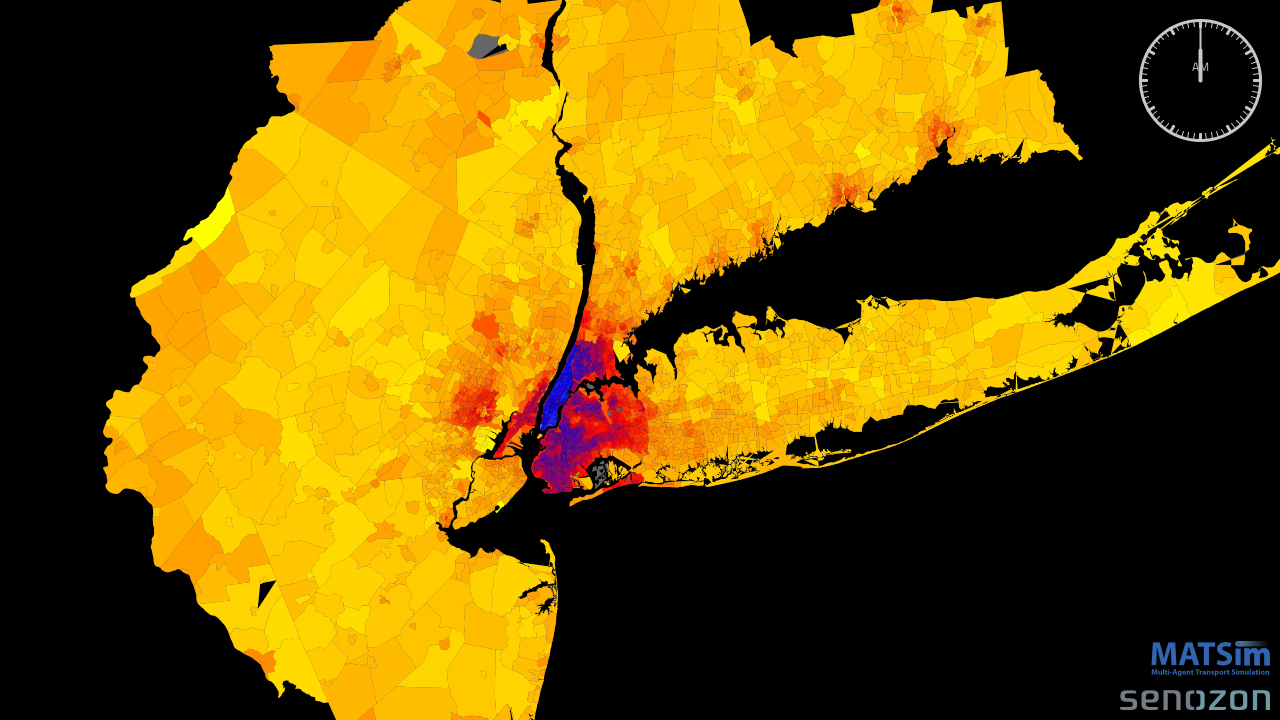
\includegraphics[width=0.95\textwidth, angle=0]{./using/figures/ny_carshare_TAZ_full.png}}%
{}

\createfigure%
{Car share (Manhattan)}%
{Car share (Manhattan)}%
{\label{fig:ny_car_share_gross}}%
{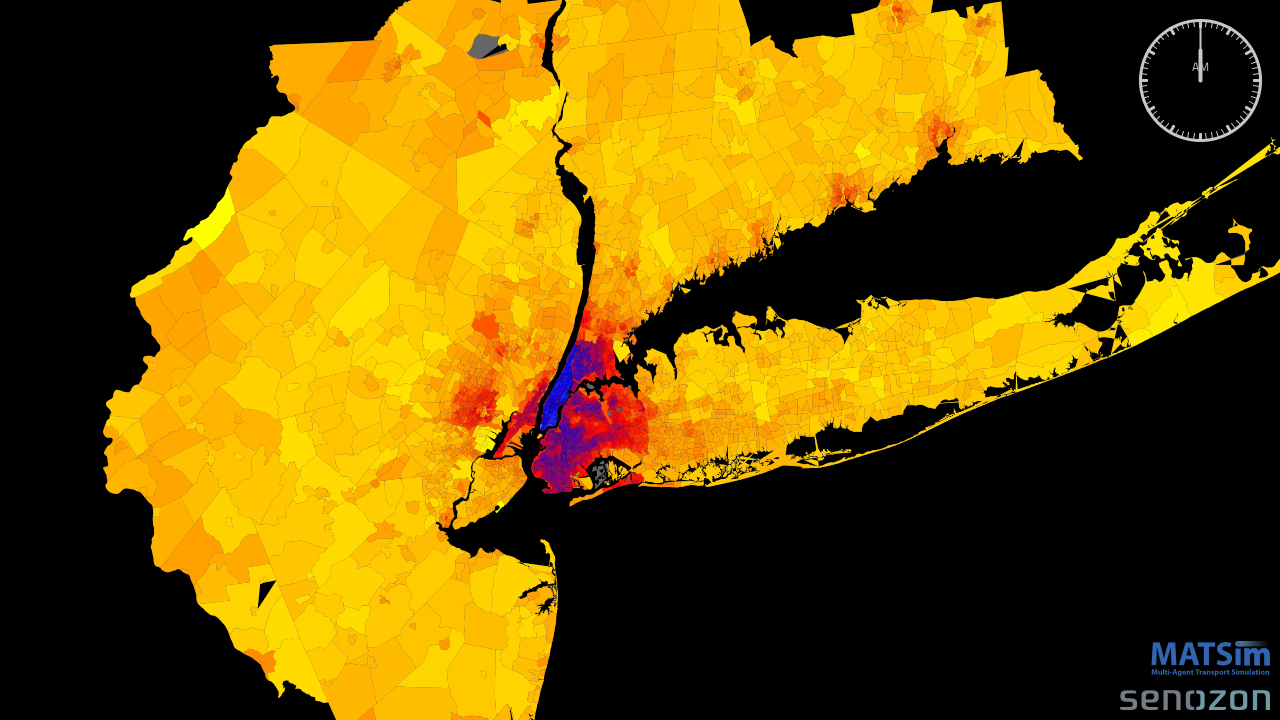
\includegraphics[width=0.95\textwidth, angle=0]{./using/figures/ny_carshare_TAZ_full.png}}%
{}

Finally, Figure~\ref{fig:ny_traffic} showed traffic flows in Lower Manhattan. Cars were represented by rectangulars, public transport vehicles by arrows. Further model outcomes were presented by \citet[][]{Balmer_unpub_ZMNY_2014}. An online movie can be found at \url{http://senozon.com/news/2014-05/zürich-meets-new-york}

\createfigure%
{Traffic flows in Lower Manhattan}%
{Traffic flows in Lower Manhattan}%
{\label{fig:ny_traffic}}%
{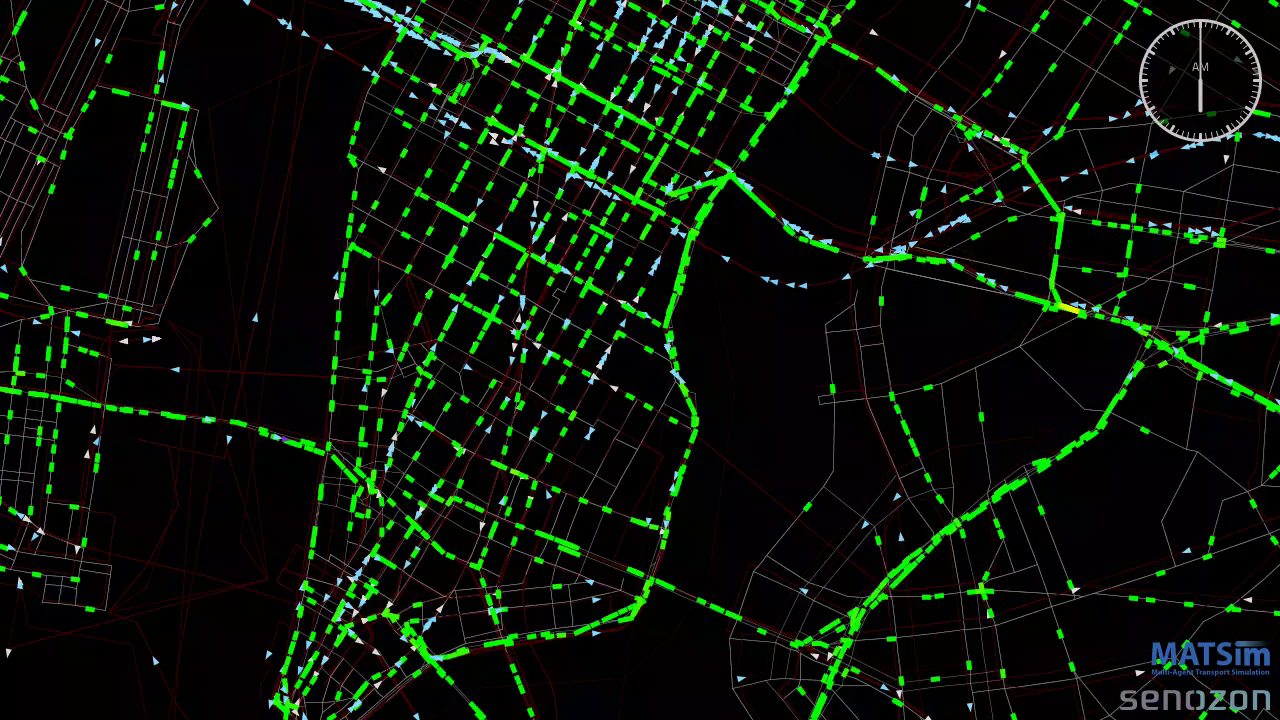
\includegraphics[width=0.95\textwidth, angle=0]{./using/figures/ny_traffic.png}}%
{}

% ##################################################################################################################